\documentclass[journal,twoside,web]{ieeecolor}
\usepackage{generic}
\usepackage{cite}
\usepackage{amsmath,amssymb,amsfonts}
\usepackage{algorithmic}
\usepackage{graphicx}
\usepackage{algorithm,algorithmic}
\usepackage{hyperref}
\hypersetup{hidelinks}
\usepackage{textcomp}
\usepackage{booktabs}
\usepackage{multirow}
\usepackage{array}
\usepackage{tabularx}
\usepackage{url}
\usepackage{balance}
\raggedbottom
\def\BibTeX{{\rm B\kern-.05em{\sc i\kern-.025em b}\kern-.08em
    T\kern-.1667em\lower.7ex\hbox{E}\kern-.125emX}}
\markboth{MediTrack: A Multi-Stakeholder Mobile Health Platform with On-Device Clinical Analytics}
{MediTrack: A Multi-Stakeholder Mobile Health Platform with On-Device Clinical Analytics}

\begin{document}
\title{MediTrack: A Multi-Stakeholder Mobile Health
Platform with On-Device Clinical Analytics and
Role-Based Security Architecture}
\author{Vijaya Wujjwal Reddy and K.~Divya
\thanks{Manuscript submitted March 2026. This work was
conducted as part of academic research in mobile health
systems development at Narayana Engineering College,
Nellore.}
\thanks{Vijaya Wujjwal Reddy is a student in the
Department of Computer Science and Engineering,
Narayana Engineering College, Nellore, India
(e-mail: wujjwalreddy@gmail.com).}
\thanks{K. Divya, M.Tech (Ph.D), is an Assistant
Professor in the Department of Computer Science and
Engineering, Narayana Engineering College, Nellore,
India. She served as the mentor for this work.}}

\maketitle
\thispagestyle{empty}

\begin{abstract}
Mobile health (mHealth) applications have emerged as
critical tools for chronic disease management, yet most
existing solutions address only a single
stakeholder---typically the patient---leaving fragmented
workflows between patients, physicians, pharmacies, and
administrators. This paper presents MediTrack, a
comprehensive multi-stakeholder Android-based health
management platform that unifies medication tracking,
vital sign monitoring, clinical decision support,
pharmacy inventory management, and real-time
doctor-patient communication under a single,
security-hardened architecture. MediTrack employs a
modular Model-View-ViewModel (MVVM) architecture with
Hilt-based dependency injection, backed by Firebase
cloud services for real-time data synchronization. A key
contribution is the on-device health analytics pipeline,
comprising five interconnected
engines---RiskScoreEngine, TrendPredictionEngine,
VitalAlertEngine, HealthInsightEngine, and
UnifiedAlertPrioritizer---that perform composite risk
scoring, consecutive-trend detection, threshold-based
vital alerting, and personalized health suggestions
without requiring server-side computation. The platform
enforces a fine-grained role-based access control (RBAC)
model with server-side Firestore security rules spanning
540 lines, implementing immutable audit trails,
state-machine-validated order workflows, and
cross-tenant data isolation. We detail the system
architecture, security model, analytics pipeline, and
multi-role workflows, and evaluate the platform through
quantitative codebase metrics and a comparative feature
analysis against existing mHealth applications.
MediTrack demonstrates that a single mobile application
can effectively serve the complete healthcare ecosystem
while maintaining clinical data integrity and privacy
through defense-in-depth security.
\end{abstract}

\begin{IEEEkeywords}
Clinical decision support, Firebase, health analytics,
medication adherence, mobile health (mHealth), MVVM
architecture, pharmacy management, role-based access
control.
\end{IEEEkeywords}

\section*{Nomenclature}
\begin{tabbing}
\hspace{2.5cm}\=\kill
ADA \> American Diabetes Association \\
AHA/ACC \> American Heart Association / \\
\> American College of Cardiology \\
CDSS \> Clinical Decision Support System \\
DI \> Dependency Injection \\
EHR \> Electronic Health Record \\
FHIR \> Fast Healthcare Interoperability \\
\> Resources \\
JNC \> Joint National Committee \\
mHealth \> Mobile Health \\
MVVM \> Model-View-ViewModel \\
RBAC \> Role-Based Access Control \\
TLS \> Transport Layer Security
\end{tabbing}

%% ================================================================
%% I. INTRODUCTION
%% ================================================================
\section{Introduction}
\label{sec:introduction}
\IEEEPARstart{T}{he} proliferation of smartphones has
created unprecedented opportunities for healthcare
delivery through mobile applications. The global mobile
health market, valued at \$68.1 billion in 2024, is
projected to reach \$362.7 billion by 2032, driven by
rising chronic disease burden, increasing smartphone
penetration, and growing demand for patient-centric
healthcare solutions \cite{grandview2024}. Despite this
growth, the mHealth landscape remains fragmented:
medication reminder applications lack clinical
oversight, electronic health record (EHR) systems
provide limited patient engagement, and pharmacy
platforms operate in isolation from clinical workflows.

Current mHealth solutions suffer from three fundamental
limitations. First, {\it stakeholder fragmentation}:
most applications serve a single user role, forcing
healthcare ecosystems to rely on multiple disconnected
tools. A patient may use one application for medication
reminders, another for health logging, and communicate
with their physician through yet another platform.
Second, {\it limited on-device intelligence}: health
analytics typically require server-side processing or
cloud-based machine learning services, introducing
latency, privacy concerns, and connectivity
dependencies. Third, {\it insufficient security
architectures}: many mHealth applications rely solely
on client-side validation, leaving clinical data
vulnerable to unauthorized access and tampering.

This paper presents MediTrack, a comprehensive mobile
health platform designed to address these limitations
through three principal contributions:

\begin{enumerate}
\item {\bf Multi-stakeholder architecture:} A unified
platform serving four distinct roles---Patient, Doctor,
Pharmacy, and Administrator---with role-specific
dashboards, workflows, and data access patterns,
eliminating the need for multiple disconnected
applications.

\item {\bf On-device health analytics pipeline:} A
modular analytics engine comprising five interconnected
components that perform composite health risk scoring,
trend prediction, vital threshold alerting, and
personalized health suggestions entirely on the mobile
device, enabling real-time clinical intelligence
without cloud computation dependencies.

\item {\bf Defense-in-depth security model:} A layered
security architecture combining server-side Firestore
security rules with role-based access control,
immutable audit trails, state-machine-validated
workflows, and cross-tenant data isolation, ensuring
clinical data integrity and compliance with healthcare
data protection principles.
\end{enumerate}

The remainder of this paper is organized as follows.
Section~\ref{sec:related} reviews related work in
mHealth platforms, clinical decision support, and
mobile security. Section~\ref{sec:architecture}
presents the overall system architecture.
Section~\ref{sec:workflows} details the multi-role
workflow design. Section~\ref{sec:analytics} describes
the on-device analytics pipeline.
Section~\ref{sec:security} elaborates on the security
architecture. Section~\ref{sec:evaluation} presents
the evaluation methodology and results.
Section~\ref{sec:discussion} discusses limitations and
future work. Section~\ref{sec:conclusion} concludes
the paper.


%% ================================================================
%% II. RELATED WORK
%% ================================================================
\section{Related Work}
\label{sec:related}

\subsection{Mobile Health Platforms}
Mobile health applications have evolved from simple
medication reminders to comprehensive health management
platforms. Medisafe \cite{medisafe} pioneered
cloud-synced medication tracking with family monitoring
capabilities but lacks clinical decision support and
pharmacy integration. MyTherapy \cite{mytherapy}
combines medication reminders with health journaling
and offers healthcare provider reporting; however, it
does not support real-time doctor-patient communication
or multi-role access control. CareZone \cite{carezone}
integrates medication management with pharmacy features
but operates as a patient-only application without
clinical decision workflows.

More comprehensive platforms have emerged in the
clinical domain. Epic MyChart \cite{mychart} extends
electronic health records to mobile devices with
appointment scheduling, messaging, and test results
access. However, MyChart functions as a patient portal
tethered to specific healthcare institutions rather
than an independent platform, and it lacks on-device
analytics or pharmacy inventory management. Apple
Health \cite{applehealth} and Google Health
Connect \cite{healthconnect} provide health data
aggregation frameworks but do not implement clinical
workflows or multi-stakeholder interaction.

\subsection{Clinical Decision Support Systems}
Clinical decision support systems (CDSS) have been
extensively studied in hospital
settings \cite{middleton2016}. Mobile CDSS
implementations typically fall into two categories:
rule-based systems that apply predefined clinical
guidelines \cite{garg2005} and machine-learning-based
systems that require cloud
infrastructure \cite{topol2019}. MediTrack's approach
occupies a middle ground: it implements evidence-based
clinical rules (blood pressure staging per JNC
guidelines, glucose thresholds per ADA standards) in a
modular on-device pipeline that can operate without
network connectivity.

Recent work on mobile clinical analytics includes
HealthAssist \cite{chen2021}, which uses smartphone
sensors for activity-based health predictions, and
VitalConnect \cite{vitalconnect}, which focuses on
continuous vital sign monitoring from wearable devices.
Unlike these specialized solutions, MediTrack's
analytics pipeline processes user-reported health logs
to generate composite risk scores, detect vital sign
trends, and produce actionable health
suggestions---functionality that does not require
specialized hardware.

\subsection{Security in mHealth Applications}
Healthcare data security remains a critical concern in
mHealth. A systematic review by Iwaya
{\it et al.} \cite{iwaya2020} found that 80\% of
surveyed health applications had significant security
vulnerabilities, including inadequate access control
and unencrypted data storage. The OWASP Mobile Security
Testing Guide \cite{owasp} provides a framework for
mobile application security assessment, emphasizing
authentication, data storage, network communication,
and platform interaction.

Firebase Security Rules, used in MediTrack's backend,
provide a declarative security model that is evaluated
server-side, preventing client-side
bypass \cite{firebase_rules}. While previous work has
documented Firebase security patterns for
general-purpose
applications \cite{sudhodanan2020}, this paper
demonstrates their application to healthcare-specific
requirements: immutable audit trails,
state-machine-validated clinical workflows, and
multi-tenant pharmacy data isolation.

\subsection{Comparison with Existing Solutions}
Table~\ref{tab:comparison} summarizes the feature
comparison between MediTrack and existing mHealth
platforms, highlighting MediTrack's unique combination
of multi-stakeholder support, on-device analytics,
and comprehensive security architecture.

\begin{table*}[!t]
\caption{Feature Comparison of mHealth Platforms}
\label{tab:comparison}
\centering\small
\begin{tabular}{l c c c c c c}
\toprule
{\bf Feature} & {\bf Medisafe} & {\bf MyTherapy}
& {\bf MyChart} & {\bf Apple H.} & {\bf CareZone}
& {\bf MediTrack} \\
\midrule
Medication Tracking & Yes & Yes & Yes
& No & Yes & {\bf Yes} \\
Health Vital Logging & No & Limited & Yes
& Yes & No & {\bf Yes} \\
Clinical Decision Support & No & No & Limited
& No & No & {\bf Yes} \\
Multi-Role RBAC & No & No & Yes$^*$
& No & No & {\bf Yes} \\
On-Device Analytics & No & No & No
& Limited & No & {\bf Yes} \\
Doctor-Patient Chat & No & No & Yes
& No & No & {\bf Yes} \\
Pharmacy Integration & No & No & No
& No & Limited & {\bf Yes} \\
Appointment Mgmt. & No & No & Yes
& No & No & {\bf Yes} \\
Prescription Versioning & No & No & Yes
& No & No & {\bf Yes} \\
Offline Support & Limited & Limited & No
& Yes & No & {\bf Yes} \\
Immutable Audit Trails & No & No & Yes$^*$
& No & No & {\bf Yes} \\
Risk Score Computation & No & No & No
& No & No & {\bf Yes} \\
\bottomrule
\multicolumn{7}{l}{\footnotesize $^*$Within
institutional deployment only.}
\end{tabular}
\end{table*}


%% ================================================================
%% III. SYSTEM ARCHITECTURE
%% ================================================================
\section{System Architecture}
\label{sec:architecture}

\subsection{Architectural Overview}
MediTrack follows the Model-View-ViewModel (MVVM)
architectural pattern, a well-established design for
Android applications that promotes separation of
concerns, testability, and lifecycle awareness.
Fig.~\ref{fig:architecture} illustrates the high-level
system architecture, comprising four principal layers:
Presentation, Domain, Data, and Infrastructure.

\begin{figure*}[!t]
\centering
% ---- REPLACE WITH YOUR GENERATED IMAGE ----
% 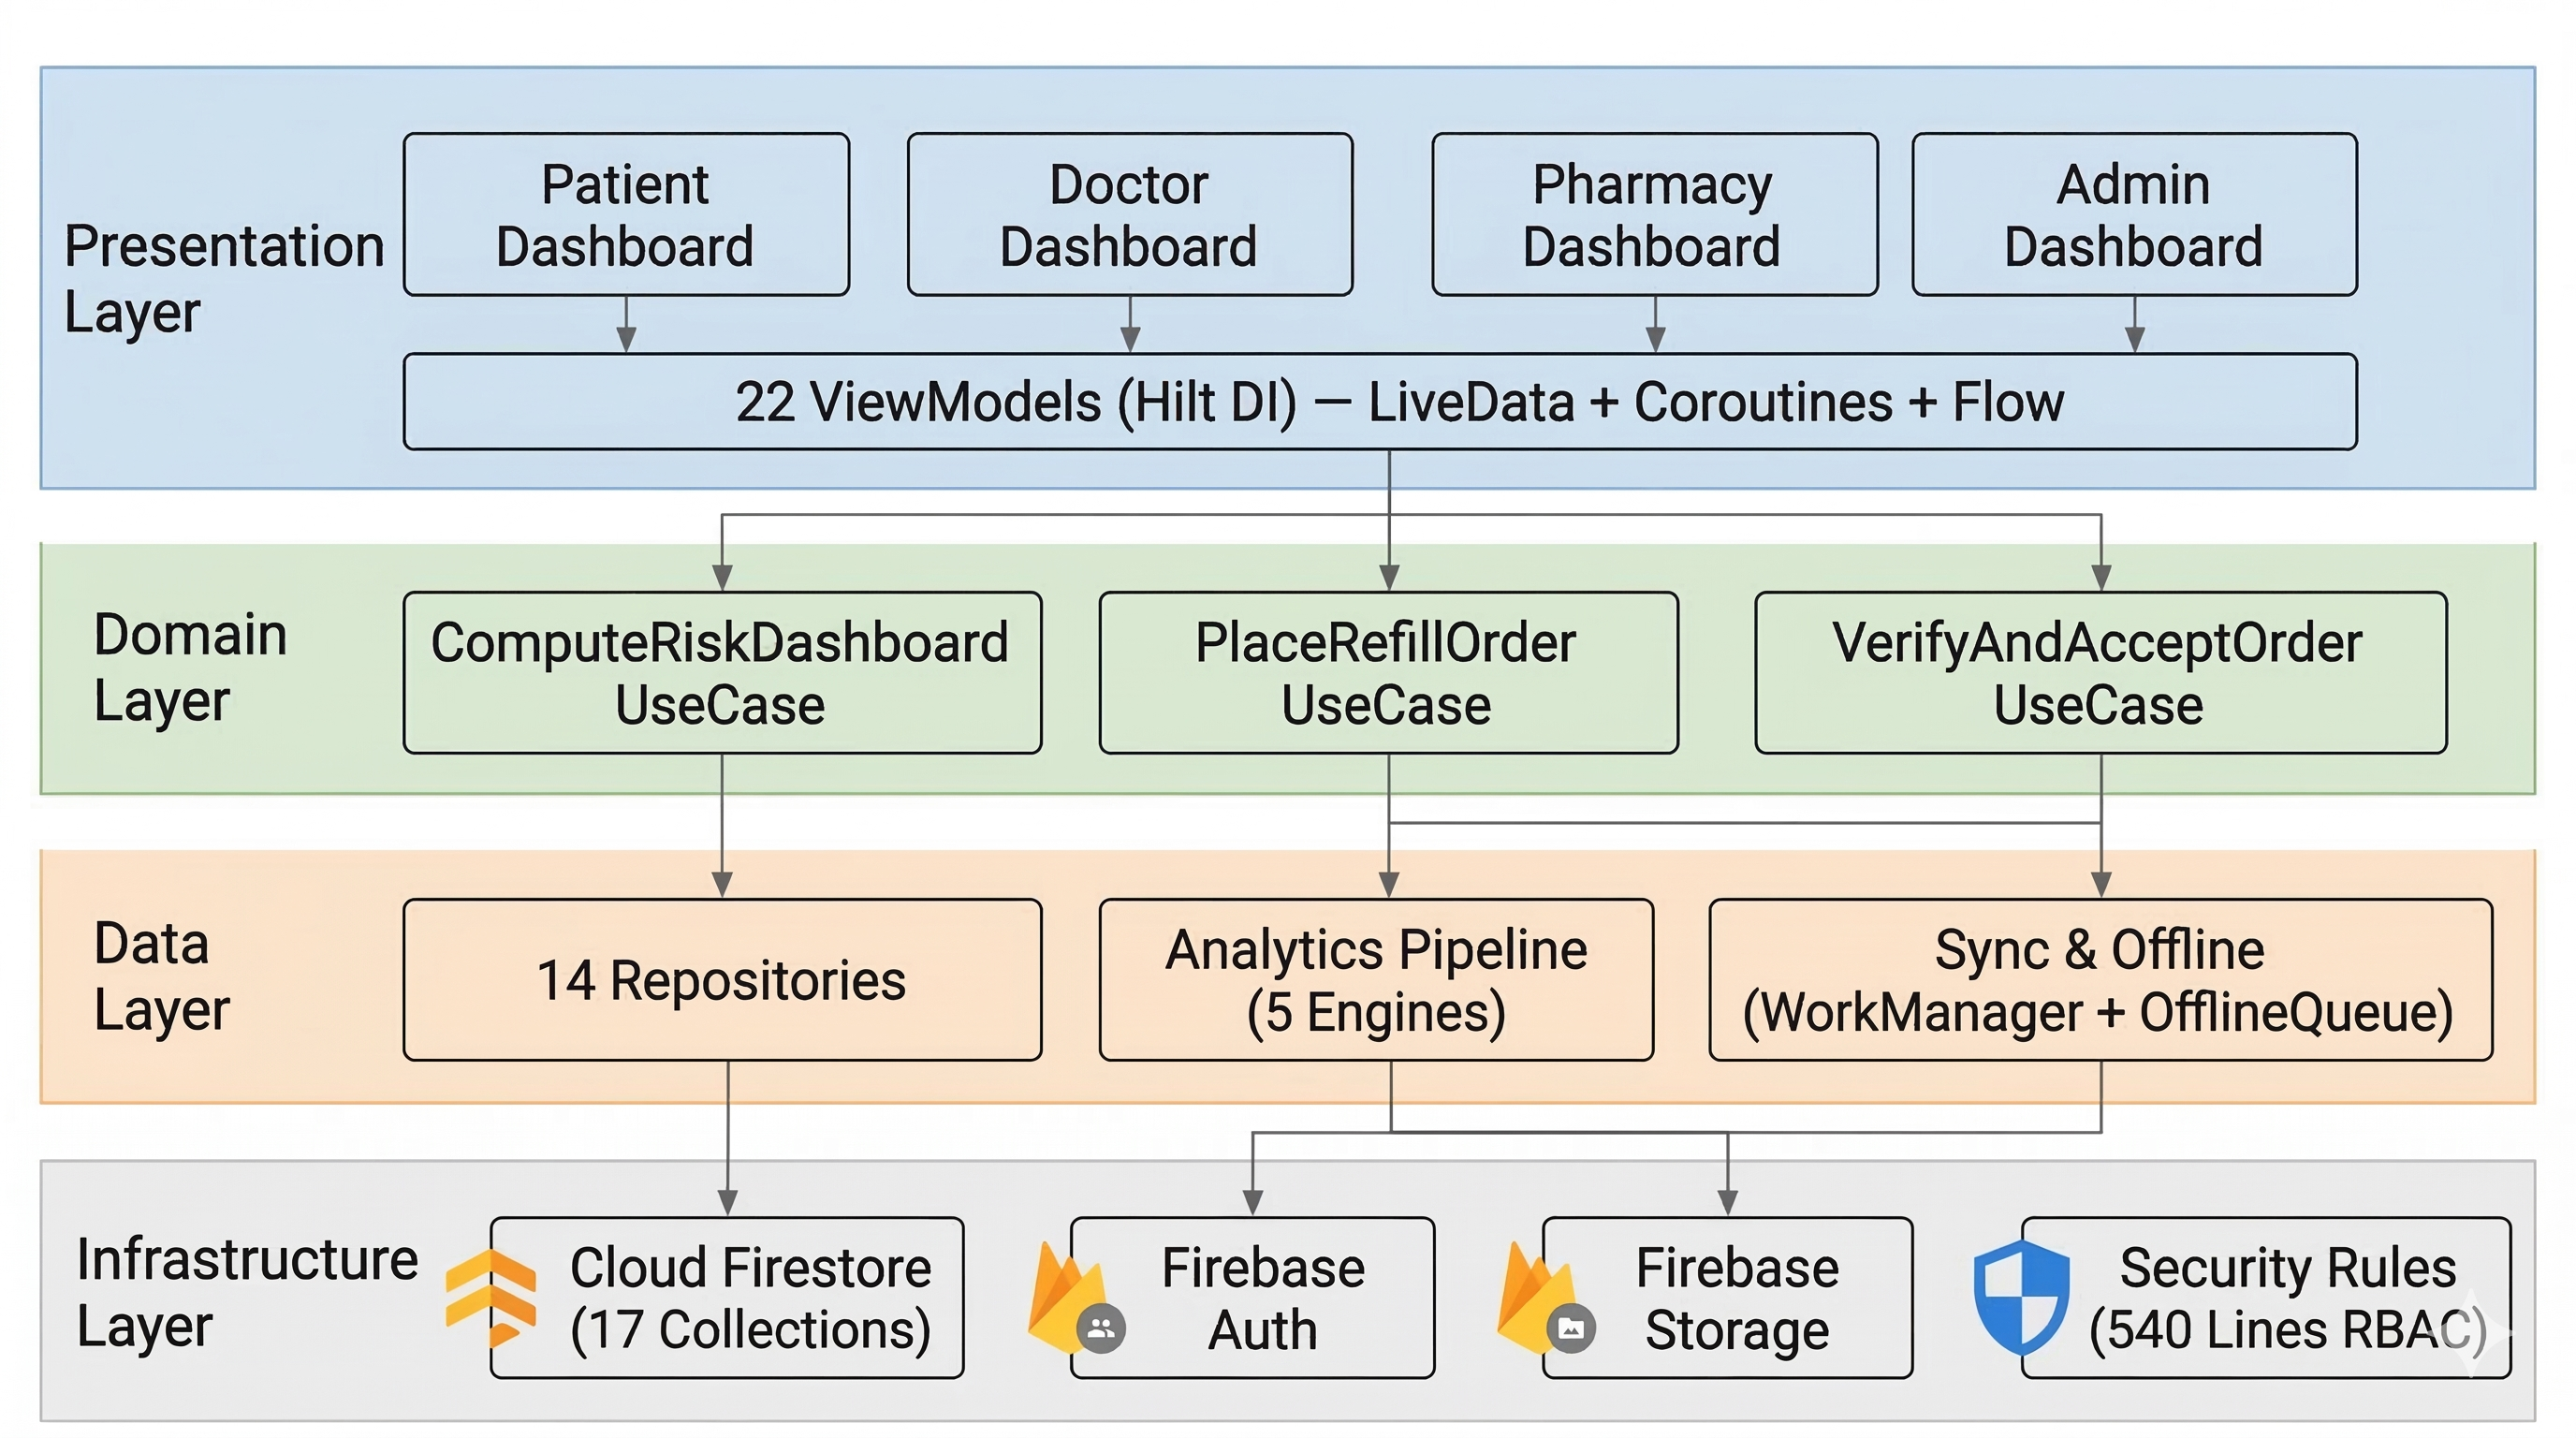
\includegraphics[width=\textwidth]{fig_architecture.png}
\fbox{\parbox{0.95\textwidth}{\centering\vspace{2.5cm}
{\bf [INSERT FIGURE 1: System Architecture Diagram]}
\vspace{2.5cm}}}
\caption{MediTrack system architecture showing the
four-layer MVVM design with Firebase infrastructure.
The Presentation Layer contains 33 Activities driven
by 22 ViewModels. The Domain Layer houses use cases
for complex multi-repository orchestration. The Data
Layer comprises 14 repositories and the analytics
pipeline. The Infrastructure Layer is built on
Firebase services with 540-line server-side security
rules.}
\label{fig:architecture}
\end{figure*}

The Presentation Layer consists of 33 Activity classes
utilizing ViewBinding for type-safe view references,
driven by 22 ViewModels that expose UI state through
LiveData observables. The Domain Layer houses use cases
that orchestrate complex multi-repository operations.
The Data Layer comprises 14 repositories serving as
the single source of truth, bridging ViewModels to the
Infrastructure Layer. The Infrastructure Layer is built
upon Firebase services including Cloud Firestore
(17 collections), Firebase Authentication, and
Firebase Storage.

\subsection{Technology Stack}
MediTrack is developed in Kotlin targeting Android
SDK~36 (minimum SDK~24, covering 98.1\% of active
devices). Table~\ref{tab:techstack} summarizes the key
technologies employed.

\begin{table}[!t]
\caption{Technology Stack}
\label{tab:techstack}
\centering\small
\begin{tabular}{p{1.8cm} p{2.6cm} p{2.5cm}}
\toprule
{\bf Component} & {\bf Technology}
& {\bf Purpose} \\
\midrule
Language & Kotlin 2.1.0
& Development lang. \\
Arch. & MVVM + Clean
& Separation of concerns \\
DI & Hilt (Dagger) + KSP
& Compile-time DI \\
Backend & Firebase Suite
& Cloud data \& auth \\
Async & Coroutines + Flow
& Reactive async \\
UI & ViewBinding
& Type-safe views \\
Charts & MPAndroidChart
& Data visualization \\
Background & WorkManager
& Periodic sync \\
Alarms & AlarmManager + Svc.
& Med. reminders \\
Offline & PersistentCache
& Offline-first access \\
Security & Firestore Rules
& Server-side RBAC \\
\bottomrule
\end{tabular}
\end{table}

\subsection{Data Model}
MediTrack's data layer comprises 17 Firestore
collections storing 17 distinct model types. The data
model was designed with three principles:
(i)~denormalization for read performance, following
Firestore best practices; (ii)~immutability for
audit-critical collections; and (iii)~role-scoped
access patterns. Fig.~\ref{fig:datamodel} presents
the entity-relationship diagram for the core data
model.

\begin{figure*}[!t]
\centering
% ---- REPLACE WITH YOUR GENERATED IMAGE ----
% \includegraphics[width=\textwidth]{fig_datamodel.png}
\fbox{\parbox{0.95\textwidth}{\centering\vspace{2.5cm}
{\bf [INSERT FIGURE 2: Entity-Relationship Diagram]}
\vspace{2.5cm}}}
\caption{Entity-relationship diagram of MediTrack's
core data model showing relationships between Users
(Patient, Doctor), HealthLogs, Medicines,
ClinicalDecisions, PrescriptionRecords, Appointments,
RefillOrders, Pharmacies, InventoryItems,
Conversations, and Messages across 17 Firestore
collections.}
\label{fig:datamodel}
\end{figure*}

Key design decisions include:

\begin{itemize}
\item {\bf Prescriptions are never deleted:} The
{\tt prescriptions} collection enforces
{\tt allow delete: if false} at the Firestore rules
level, preserving a complete audit trail of all
medical prescriptions.

\item {\bf Medicine intakes are immutable:} Once a
patient records taking a medication, the record
cannot be modified or deleted, ensuring adherence
data integrity.

\item {\bf Multi-doctor support:} Users maintain an
{\tt assignedDoctors} array, enabling multiple
physicians to access a patient's
records---reflecting the reality that patients often
see multiple specialists.
\end{itemize}

\subsection{Dependency Injection Architecture}
MediTrack employs Hilt, Google's recommended dependency
injection framework for Android, configured with two
primary modules. {\tt FirebaseModule} provides singleton
instances of {\tt FirebaseAuth},
{\tt FirebaseFirestore}, and {\tt FirebaseStorage},
ensuring a single connection pool throughout the
application lifecycle. {\tt RepositoryModule} binds all
14 repository implementations as singletons, receiving
Firebase instances via constructor injection.

ViewModels are annotated with {\tt @HiltViewModel} and
declare repository dependencies in their constructors,
enabling automated injection. This architecture ensures
that repositories maintain a single instance throughout
the application lifecycle, preventing duplicate
Firestore listeners and reducing memory consumption.


%% ================================================================
%% IV. MULTI-ROLE WORKFLOW DESIGN
%% ================================================================
\section{Multi-Role Workflow Design}
\label{sec:workflows}

\subsection{Role-Based Navigation}
MediTrack implements a four-role system reflecting the
primary stakeholders in an outpatient healthcare
ecosystem. Upon successful authentication, a
{\tt RoleBasedNavigator} component directs users to
role-specific entry points based on their Firestore
user document: PATIENT to
{\tt HomeDashboardActivity}, DOCTOR to
{\tt DoctorDashboardActivity}, ADMIN to
{\tt AdminDashboardActivity}, and PHARMACY to
{\tt PharmacyDashboardActivity}.
Fig.~\ref{fig:navigation} illustrates this flow.

\begin{figure}[!t]
\centering
% ---- REPLACE WITH YOUR GENERATED IMAGE ----
% \includegraphics[width=\columnwidth]{fig_navigation.png}
\fbox{\parbox{0.9\columnwidth}{\centering\vspace{3cm}
{\bf [INSERT FIGURE 3: Role-Based Navigation Flow]}
\vspace{3cm}}}
\caption{Role-based navigation flow showing
authentication, role detection, approval verification,
and role-specific dashboard routing for all four user
types. Doctor and Pharmacy roles require explicit
admin approval.}
\label{fig:navigation}
\end{figure}

Doctor and Pharmacy accounts require explicit
administrator approval before accessing protected
features. Unapproved accounts are directed to
{\tt AccountPendingActivity}, and the Firestore
security rules enforce this requirement server-side
through the {\tt isApproved()} helper function, which
explicitly checks for an ``APPROVED'' status
field---missing status values are never treated as
approved.

\subsection{Patient Workflows}
The patient role encompasses five primary workflows:

{\bf 1) Medication Management:} Patients add
medications with name, dosage, frequency, unit, and
reminder times. The system schedules exact alarms via
Android's {\tt AlarmManager}, which trigger a chain
of {\tt BroadcastReceiver} $\rightarrow$
{\tt ForegroundService} $\rightarrow$ Notification
with full-screen intent. Medication intake is tracked
through an immutable {\tt medicineIntakes} collection,
and adherence percentage is computed in real-time. A
{\tt BootReceiver} reschedules all alarms after device
restart.

{\bf 2) Health Vital Logging:} Patients record vital
signs including blood pressure (systolic/diastolic),
heart rate, glucose level, temperature, weight, and
oxygen saturation. Each entry can include symptom tags
and free-text notes. Upon entry, the
{\tt VitalAlertEngine} evaluates readings against
clinical thresholds and generates immediate alerts
for abnormal values.

{\bf 3) Appointment Booking:} Patients view available
doctor time slots, book appointments (consultation,
follow-up, emergency, or routine checkup), and receive
appointment reminders. The system prevents
double-booking through availability slot management.

{\bf 4) Medicine Refill Ordering:} Patients can order
medication refills through integrated pharmacies. The
order lifecycle follows a state machine: PENDING
$\rightarrow$ CONFIRMED $\rightarrow$ PREPARING
$\rightarrow$ SHIPPED $\rightarrow$ DELIVERED, with
server-side validation ensuring only valid transitions
occur.

{\bf 5) Health Insights Dashboard:} Patients access a
risk dashboard displaying their composite health risk
score (0--100), vital sign trends, personalized health
suggestions, and active alerts---all computed on-device
by the analytics pipeline described in
Section~\ref{sec:analytics}.

\subsection{Doctor Workflows}
{\bf 1) Patient Management:} Doctors view a list of
assigned patients with key indicators including latest
vitals, adherence rate, and risk category. Doctors can
access patient health logs, medication lists, and
intake history.

{\bf 2) Clinical Decision Support:} Doctors create
clinical decisions spanning seven types:
{\it Prescription}, {\it Follow-Up},
{\it Vital Alert}, {\it Recommendation},
{\it Diagnosis}, {\it Lab Order}, and
{\it Lifestyle}. Prescriptions include structured
fields for medication name, dosage, frequency, route,
unit, duration, and instructions, drawn from
standardized medical reference lists.

{\bf 3) Prescription Management:} Prescriptions follow
a versioned lifecycle (ACTIVE $\rightarrow$ MODIFIED
$\rightarrow$ STOPPED $\rightarrow$ COMPLETED). Each
modification generates a {\tt VersionEntry} recording
changed fields, previous values, change notes, and
the modifying physician---ensuring a complete history
of prescription changes.

{\bf 4) Doctor Notes:} Physicians can create public
notes (visible to the patient) and private notes
(visible only to the authoring doctor and
administrators), supporting both patient communication
and internal clinical documentation.

\subsection{Pharmacy Workflows}
{\bf 1) Inventory Management:} Pharmacies manage their
medicine inventory with real-time stock tracking,
including stock quantities, unit prices, expiry dates,
batch numbers, and low-stock thresholds. Inventory
items use a soft-delete pattern ({\tt isActive} flag)
to preserve historical references.

{\bf 2) Order Fulfillment:} Pharmacies receive refill
orders and advance them through the order state
machine. The {\tt VerifyAndAcceptOrderUseCase} handles
prescription verification for controlled medications
before allowing order acceptance.

{\bf 3) Transaction History:} All completed order
transactions are recorded immutably, including the
amount, prescription verification status, and
associated order and pharmacy identifiers.

\subsection{Administrator Workflows}
Administrators perform user management (approve/reject
doctor and pharmacy accounts), monitor system activity
through audit logs, and have read access to all orders.
Critically, the ADMIN role cannot be created through
client SDKs---the Firestore rules restrict user
creation to PATIENT, DOCTOR, and PHARMACY roles,
requiring server-side Firebase Admin SDK operations
for admin account provisioning.


%% ================================================================
%% V. ON-DEVICE HEALTH ANALYTICS PIPELINE
%% ================================================================
\section{On-Device Health Analytics Pipeline}
\label{sec:analytics}

\subsection{Pipeline Overview}
MediTrack's analytics pipeline is a central
contribution of this work. Unlike cloud-dependent
analytics systems, the pipeline executes entirely
on-device, providing three key advantages:
(i)~zero-latency health insights, (ii)~privacy
preservation by keeping sensitive health data local
during computation, and (iii)~offline availability.
The pipeline is orchestrated by the
{\tt InsightEngine} facade, which coordinates five
specialized engines. Fig.~\ref{fig:analytics}
illustrates the pipeline architecture.

\begin{figure*}[!t]
\centering
% ---- REPLACE WITH YOUR GENERATED IMAGE ----
% \includegraphics[width=\textwidth]{fig_analytics.png}
\fbox{\parbox{0.95\textwidth}{\centering\vspace{2.5cm}
{\bf [INSERT FIGURE 4: Analytics Pipeline]}
\vspace{2.5cm}}}
\caption{On-device health analytics pipeline
architecture. The {\tt InsightEngine} facade
coordinates the {\tt RiskScoreEngine} (composite
0--100 scoring), {\tt TrendPredictionEngine}
(consecutive pattern detection with linear
regression), and {\tt VitalAlertEngine}
(threshold-based vital alerts). Outputs are unified
by the {\tt UnifiedAlertPrioritizer} and fed to the
{\tt HealthInsightEngine} for personalized suggestion
generation.}
\label{fig:analytics}
\end{figure*}

\subsection{RiskScoreEngine: Composite Health Risk
Scoring}
The {\tt RiskScoreEngine} computes a composite health
risk score ranging from 0 to 100 through weighted
multi-dimensional analysis. The score integrates four
dimensions, each reflecting a distinct aspect of
patient health, as shown in
Table~\ref{tab:riskweights}.

\begin{table}[!t]
\caption{Risk Score Dimension Weights}
\label{tab:riskweights}
\centering\small
\begin{tabular}{p{2.2cm} c p{3.2cm}}
\toprule
{\bf Dimension} & {\bf Wt.}
& {\bf Description} \\
\midrule
Vital Signs (BP, HR, Glucose, Temp) & 40\%
& Clinical thresholds per medical guidelines \\
Medication Adherence & 25\%
& Inverted adherence \% (100\% = 0 risk) \\
Symptom Burden & 20\%
& Severity-weighted (severe=25, mod.=12, mild=5) \\
Data Recency \& Completeness & 15\%
& Days since last log, weekly frequency \\
\bottomrule
\end{tabular}
\end{table}

The Vital Signs dimension evaluates blood pressure,
heart rate, glucose, and temperature against clinically
established thresholds. Blood pressure scoring follows
the Joint National Committee (JNC) staging guidelines
as shown in Table~\ref{tab:bpscoring}.

\begin{table}[!t]
\caption{Blood Pressure Risk Scoring Thresholds}
\label{tab:bpscoring}
\centering\small
\begin{tabular}{c c c l}
\toprule
{\bf Sys.} & {\bf Dia.} & {\bf Score}
& {\bf Clinical Stage} \\
{\bf (mmHg)} & {\bf (mmHg)} & & \\
\midrule
$\geq$180 & $\geq$120 & 100
& Hypertensive Crisis \\
$\geq$160 & $\geq$100 & 85
& Stage 2+ Hypertension \\
$\geq$140 & $\geq$90  & 70
& Stage 1 Hypertension \\
$\geq$130 & $\geq$85  & 50
& Elevated \\
80--129   & 50--84    & 0--30
& Normal Range \\
$<$80     & $<$50     & 80
& Dangerously Low \\
\bottomrule
\end{tabular}
\end{table}

Glucose scoring follows American Diabetes Association
(ADA) thresholds, with severe hyperglycemia
($\geq$300~mg/dL) scoring 100, very high ($\geq$200)
scoring 85, diabetic range ($\geq$126) scoring 60,
pre-diabetic (100--125) scoring 30, hypoglycemia
($<$70) scoring 75, and severe hypoglycemia ($<$54)
scoring 95.

The engine applies four multi-factor correlation rules
that add bonus risk points when multiple adverse
factors co-occur:

\begin{itemize}
\item {\it Metabolic Syndrome Risk} (+10 points):
High BP + elevated glucose + poor adherence.
\item {\it Cardiac Stress} (+12 points):
Elevated BP + elevated HR + chest pain symptoms.
\item {\it Uncontrolled Diabetic Risk} (+8 points):
High glucose + poor adherence.
\item {\it Symptomatic Non-Adherence} (+5 points):
Recurring symptoms + missed medications.
\end{itemize}

The composite risk score $R$ is computed as:
\begin{equation}
R = \min\!\left(100,\; \sum_{i=1}^{4} w_i \cdot d_i
+ \sum_{j=1}^{4} c_j\right)
\label{eq:riskscore}
\end{equation}
where $w_i$ and $d_i$ represent the weight and
normalized score (0--100) of each dimension, and
$c_j$ represents the correlation bonus for each
multi-factor rule. The final score is categorized
into four risk levels: LOW (0--25), MODERATE (26--50),
HIGH (51--75), and CRITICAL (76--100).

\subsection{TrendPredictionEngine: Consecutive Pattern
Detection}
The {\tt TrendPredictionEngine} detects directional
trends in six vital sign types: heart rate, systolic
blood pressure, diastolic blood pressure, glucose,
weight, and temperature. For each vital type, the
engine examines chronologically ordered readings and
counts consecutive increases or decreases. A change
exceeding 1.5\% between adjacent readings qualifies
as directional. Three or more consecutive directional
changes trigger a trend alert; five or more trigger
an accelerating trend alert.

When a trend is detected, a simple linear regression
model is fit to the trending values to project the
next expected reading. Given $n$ trending values
$(x_1, y_1), \ldots, (x_n, y_n)$, the projected
value is:
\begin{equation}
\hat{y}_{n+1} = \bar{y} + b(x_{n+1} - \bar{x})
\label{eq:regression}
\end{equation}
where $b = \frac{\sum_{i=1}^{n}(x_i - \bar{x})
(y_i - \bar{y})}{\sum_{i=1}^{n}(x_i -
\bar{x})^2}$ is the regression slope.

This approach deliberately avoids complex machine
learning models in favor of interpretable,
deterministic algorithms that can be validated against
clinical intuition and operate without training data.

\subsection{VitalAlertEngine: Real-Time Threshold
Alerting}
The {\tt VitalAlertEngine} evaluates individual health
log readings against clinically informed thresholds to
generate immediate alerts. The engine classifies each
reading into one of three severity levels: NORMAL,
WARNING, or CRITICAL. Table~\ref{tab:vitalalerts}
presents the threshold values for each vital type.

\begin{table}[!t]
\caption{Vital Alert Engine Threshold Values}
\label{tab:vitalalerts}
\centering\small
\begin{tabular}{l c c c c}
\toprule
{\bf Vital} & {\bf Crit.} & {\bf Warn.}
& {\bf Warn.} & {\bf Crit.} \\
{\bf Sign} & {\bf High} & {\bf High}
& {\bf Low} & {\bf Low} \\
\midrule
BP (mmHg) & $\geq$180/ & $\geq$140/
& $<$90/ & $<$80/ \\
& 120 & 90 & 60 & 50 \\
Glucose & $\geq$300 & $\geq$200
& $<$70 & $<$54 \\
HR (bpm) & $\geq$150 & $\geq$120
& $<$60 & $<$40 \\
Temp ($^\circ$C) & $\geq$39.5 & $\geq$38.0
& $<$36.0 & $<$35.0 \\
\bottomrule
\end{tabular}
\end{table}

\subsection{HealthInsightEngine: Personalized Health
Suggestions}
The {\tt HealthInsightEngine} generates up to eight
prioritized, actionable health suggestions by
synthesizing outputs from the other engines.
Suggestions are categorized by action type: LIFESTYLE,
MEDICATION, DOCTOR\_VISIT, MONITORING, and EMERGENCY.
Suggestions are drawn from six sources:

\begin{enumerate}
\item {\it Risk-based:} CRITICAL risk triggers ``Seek
Medical Attention''; HIGH risk triggers ``Schedule a
Doctor Visit.''
\item {\it Trend-based:} Rising vital patterns with
specific behavioral recommendations.
\item {\it Adherence-based:} Adherence below 50\%
triggers high-priority warnings.
\item {\it Vital-specific:} Metabolic risk detection
for concurrent high BP and glucose.
\item {\it Data quality:} Prompts for missing or
stale health data.
\item {\it Positive reinforcement:} Congratulatory
feedback for low risk with high adherence.
\end{enumerate}

\subsection{UnifiedAlertPrioritizer: Cross-Engine
Alert Fusion}
The {\tt UnifiedAlertPrioritizer} addresses the
challenge of heterogeneous alert formats across
engines. It maps four distinct priority taxonomies
({\tt AlertSeverity}, {\tt TrendPriority},
{\tt FactorSeverity}, {\tt SuggestionPriority}) to a
common six-level {\tt UnifiedPriority} scale:
INFORMATIONAL, LOW, MODERATE, HIGH, URGENT, and
EMERGENCY. The prioritizer deduplicates alerts by
identifier prefix (retaining the highest-severity
instance) and sorts results in descending priority
order.

\subsection{Supporting Components}
{\bf PredictiveAlertManager} prevents alert fatigue
by implementing a 24-hour debounce window per alert
type using {\tt SharedPreferences}. If the same alert
condition persists across multiple analytics runs
within the window, only the first instance generates
a notification.

{\bf ReminderOptimizer} analyzes medication intake
patterns to suggest optimal reminder times. The
algorithm compares actual intake timestamps against
scheduled reminders, identifies time slots with less
than 60\% adherence, suggests meal-aligned
alternatives (08:00, 13:00, 20:00) for better
adherence, detects over-scheduling (more than 3
medications at the same time), and flags inconvenient
timing (before 06:00 or after 23:00).


%% ================================================================
%% VI. SECURITY ARCHITECTURE
%% ================================================================
\section{Security Architecture}
\label{sec:security}

\subsection{Defense-in-Depth Model}
MediTrack implements a layered security architecture
that addresses threats at multiple levels.
Fig.~\ref{fig:security} illustrates the security
stack, comprising Application, Transport, and Server
layers.

\begin{figure}[!t]
\centering
% ---- REPLACE WITH YOUR GENERATED IMAGE ----
% \includegraphics[width=\columnwidth]{fig_security.png}
\fbox{\parbox{0.9\columnwidth}{\centering\vspace{3cm}
{\bf [INSERT FIGURE 5: Security Architecture]}
\vspace{3cm}}}
\caption{MediTrack defense-in-depth security
architecture. The Application Layer enforces backup
prevention, encrypted local storage, and client-side
audit logging. The Transport Layer provides TLS
encryption via Firebase SDK. The Server Layer
implements 540-line Firestore Security Rules with
RBAC, state machine validation, immutable audit
trails, and cross-tenant isolation.}
\label{fig:security}
\end{figure}

\subsection{Firestore Security Rules: Server-Side RBAC}
The Firestore security rules (540 lines) implement
comprehensive role-based access control through 11
helper functions. Key security patterns include:

{\bf 1) Role Verification:} Each protected operation
verifies both the user's role and their approval
status through composite helper functions such as
{\tt isApprovedDoctor()}, which combines
authentication, role, and status checks.

{\bf 2) Cross-Tenant Isolation:} Pharmacy data is
isolated through ownership verification via
{\tt isPharmacyOwner(pharmacyId)}, which
cross-references the requesting user against the
pharmacy's {\tt ownerId} field.

{\bf 3) Doctor-Patient Assignment Verification:}
Access to patient clinical data requires an
established doctor-patient relationship, verified
through the
{\tt isDoctorAssignedToPatient(patientId)} function
that checks membership in the patient's
{\tt assignedDoctors} array.

{\bf 4) Self-Privilege Escalation Prevention:} Users
cannot modify their own role or status after account
creation, and the ADMIN role cannot be assigned
through client SDKs.

\subsection{Data Immutability Guarantees}
Five collections enforce immutability at the server
level, as summarized in Table~\ref{tab:immutability}.

\begin{table}[!t]
\caption{Immutable Collection Policies}
\label{tab:immutability}
\centering\small
\begin{tabular}{l l l}
\toprule
{\bf Collection} & {\bf Policy}
& {\bf Rationale} \\
\midrule
prescriptions & Never deleted
& Audit trail \\
medicineIntakes & No update/del.
& Adherence integrity \\
auditLogs & Append-only
& Tamper-proof logs \\
transactions & No update/del.
& Financial integrity \\
riskScores & Append-only
& Temporal tracking \\
\bottomrule
\end{tabular}
\end{table}

\subsection{State Machine Validation}
Order and appointment status transitions are validated
server-side, preventing invalid workflow jumps. For
orders, valid transitions are: PENDING $\rightarrow$
CONFIRMED or CANCELLED, CONFIRMED $\rightarrow$
PREPARING or CANCELLED, PREPARING $\rightarrow$
SHIPPED, and SHIPPED $\rightarrow$ DELIVERED. This
server-side enforcement prevents malicious clients
from bypassing the intended workflow sequence.

\subsection{Data Validation}
Input validation is enforced server-side for critical
data types, including string length limits (email:
1--320 characters, display name: 1--100 characters,
medication name: 1--200 characters), required field
presence, and enum value constraints. This server-side
validation complements client-side checks, ensuring
data integrity even if the client application is
modified.


%% ================================================================
%% VII. EVALUATION
%% ================================================================
\section{Evaluation}
\label{sec:evaluation}

\subsection{Quantitative Codebase Metrics}
Table~\ref{tab:metrics} presents quantitative metrics
characterizing the MediTrack codebase, demonstrating
the substantial engineering scope of the platform.

\begin{table}[!t]
\caption{Codebase Metrics}
\label{tab:metrics}
\centering
\begin{tabular}{l r}
\toprule
{\bf Metric} & {\bf Value} \\
\midrule
Total Kotlin source files       & 148 \\
Total lines of Kotlin code      & $\sim$26,753 \\
Layout XML files                & 74 \\
Activity classes                & 33 \\
ViewModel classes               & 22 \\
Repository classes              & 14 \\
Data model classes              & 17 \\
Analytics engine classes        & 9 \\
Firestore collections           & 17 \\
Security rule helper functions  & 11 \\
Security rules (lines)          & 540 \\
Domain use cases                & 3 \\
Notification channels           & 3 \\
User roles                      & 4 \\
Clinical decision types         & 7 \\
Order status states             & 6 \\
Min SDK / Target SDK            & 24 / 36 \\
\bottomrule
\end{tabular}
\end{table}

\subsection{Architecture Quality Assessment}
We evaluate MediTrack's architecture against
established software quality attributes:

{\bf 1) Modularity:} The MVVM architecture with
dependency injection achieves high modularity. Each
feature area (medicine, health logs, appointments,
pharmacy) is encapsulated in dedicated packages with
clear boundaries. The 14 repositories provide
well-defined data access interfaces.

{\bf 2) Separation of Concerns:} The four-layer
architecture (Presentation, Domain, Data,
Infrastructure) ensures that UI logic, business
rules, data access, and platform concerns remain
decoupled. ViewModels contain no direct Firebase
references, communicating exclusively through
repository abstractions.

{\bf 3) Security Coverage:} Server-side security
rules cover all 17 collections with role-specific
access patterns. Five collections enforce
immutability. Two collections implement
state-machine validation. Client-side security
includes backup prevention and encrypted local
storage.

{\bf 4) Offline Resilience:} The dual offline
strategy (100~MB Firestore {\tt PersistentCache}
plus {\tt SharedPreferences}-based
{\tt OfflineQueueManager}) enables continued
operation without network connectivity.
{\tt WorkManager}-based periodic synchronization at
15-minute intervals ensures eventual consistency.

\subsection{Feature Coverage Analysis}
Table~\ref{tab:coverage} compares MediTrack's feature
coverage with the requirements identified in recent
mHealth literature
surveys \cite{free2013, batista2020}.

\begin{table*}[!t]
\caption{Feature Coverage vs.\ mHealth Requirements}
\label{tab:coverage}
\centering\small
\begin{tabular}{p{3.2cm} l l}
\toprule
{\bf Requirement} & {\bf Feature}
& {\bf MediTrack Implementation} \\
\midrule
\multirow{4}{*}{Medication Mgmt.}
& Reminder scheduling
& ExactAlarm + ForegroundService \\
& Adherence tracking
& Immutable intake records \\
& Low stock alerts
& Threshold-based detection \\
& Refill ordering
& State machine workflow \\
\midrule
\multirow{4}{*}{Health Monitoring}
& Vital sign logging
& 6 vital types + symptoms \\
& Trend detection
& Consecutive + lin. regression \\
& Risk assessment
& Composite 0--100 (4 dims.) \\
& Threshold alerts
& Evidence-based thresholds \\
\midrule
\multirow{3}{*}{Clinical Support}
& Prescription mgmt.
& Versioned, immutable records \\
& Clinical decisions
& 7 decision types \\
& Doctor notes
& Public + private \\
\midrule
\multirow{3}{*}{Communication}
& Doctor-patient chat
& Real-time Firestore messaging \\
& Read receipts
& Per-message tracking \\
& Appt.\ scheduling
& 4 appointment types \\
\midrule
\multirow{3}{*}{Pharmacy}
& Inventory mgmt.
& Real-time, soft-delete pattern \\
& Order fulfillment
& 6-state machine \\
& Rx verification
& Domain use case driven \\
\midrule
\multirow{3}{*}{Security}
& Authentication
& Email/password + Google OAuth \\
& Authorization
& 4 roles, server-side RBAC \\
& Audit trail
& Immutable, append-only \\
\midrule
\multirow{2}{*}{Offline Support}
& Offline data access
& 100~MB persistent cache \\
& Background sync
& WorkManager, 15-min interval \\
\bottomrule
\end{tabular}
\end{table*}

\subsection{Analytics Pipeline Evaluation}
To evaluate the analytics pipeline's clinical
alignment, we compared MediTrack's threshold values
against published clinical guidelines. Blood pressure
thresholds align with AHA/ACC 2017
guidelines \cite{whelton2018}. Glucose thresholds
align with ADA 2024 Standards of
Care \cite{ada2024}. Heart rate thresholds align with
standard clinical ranges \cite{perkins2021}.
Temperature thresholds align with WHO fever
classification \cite{who2014}. The multi-factor
correlation rules (metabolic syndrome risk, cardiac
stress, uncontrolled diabetic risk) are based on
established clinical associations documented in
medical literature \cite{grundy2004, cannon2007}.


%% ================================================================
%% VIII. DISCUSSION
%% ================================================================
\section{Discussion}
\label{sec:discussion}

\subsection{Key Contributions}
MediTrack demonstrates that a mobile-first,
multi-stakeholder health platform can achieve
comprehensive feature coverage while maintaining
architectural quality and security rigor. Three
aspects warrant further discussion.

{\bf On-device analytics as a viable alternative:}
The analytics pipeline's deterministic, rule-based
approach offers advantages over cloud-based ML:
interpretability (physicians can understand why a
risk score was assigned), reproducibility (same inputs
always produce same outputs), and privacy (no health
data leaves the device for analytics). While machine
learning approaches may achieve higher predictive
accuracy for specific tasks, the rule-based approach
is more amenable to clinical validation and regulatory
approval.

{\bf Server-side security as primary defense:} By
enforcing access control, data immutability, and
workflow validation in Firestore Security Rules,
MediTrack ensures that security cannot be bypassed
through client-side manipulation---an approach
aligned with the zero-trust security model. The
540-line rule set demonstrates that declarative
security rules can express complex healthcare access
patterns including multi-tenant isolation and state
machine validation.

{\bf Unified stakeholder platform:} The four-role
architecture eliminates data silos between care
participants. A prescription created by a doctor is
immediately visible to the patient and the fulfilling
pharmacy, with every status change audited and
validated. This unified approach reduces the
coordination overhead inherent in multi-application
healthcare ecosystems.

\subsection{Limitations}
\begin{enumerate}
\item {\it No clinical trial validation:} While the
analytics thresholds are sourced from established
guidelines, the composite risk scoring algorithm has
not been validated through a clinical trial. Future
work should conduct a prospective study comparing
MediTrack's risk assessments against clinician
judgments.

\item {\it Limited interoperability:} MediTrack uses
a Firebase-specific data model without HL7 FHIR or
openEHR support, limiting integration with existing
healthcare IT infrastructure.

\item {\it No end-to-end encryption for chat:} While
messages are encrypted in transit (TLS) and at rest
(Firestore server-side encryption), the platform
does not implement end-to-end encryption for
doctor-patient communication.

\item {\it Single-platform implementation:} The
current implementation targets Android only. A
cross-platform approach using Kotlin Multiplatform
or Flutter would broaden accessibility.

\item {\it Rule-based analytics limitations:} The
deterministic analytics pipeline cannot learn from
individual patient patterns or population-level
data. Integration with federated learning or
on-device ML models could enhance personalization
while preserving privacy.
\end{enumerate}

\subsection{Future Work}
Based on the identified limitations, we outline the
following directions:

\begin{enumerate}
\item {\bf Clinical validation study:} Conduct a
multi-site prospective study to validate the
composite risk score against clinician assessments
and patient outcomes.
\item {\bf HL7 FHIR integration:} Implement FHIR
resource mappings for interoperability with hospital
EHR systems and health information exchanges.
\item {\bf Federated learning:} Integrate on-device
federated learning to improve analytics
personalization without centralizing patient data.
\item {\bf Wearable device integration:} Extend the
health log input pipeline to accept continuous data
streams from wearables via the Health Connect API.
\item {\bf Cloud Functions:} Migrate critical business
logic (prescription verification, order processing)
to Firebase Cloud Functions for additional
server-side enforcement.
\item {\bf Cross-platform expansion:} Extend the
platform to iOS using Kotlin Multiplatform for shared
business logic.
\end{enumerate}


%% ================================================================
%% IX. CONCLUSION
%% ================================================================
\section{Conclusion}
\label{sec:conclusion}

This paper presented MediTrack, a multi-stakeholder
mobile health platform that addresses the critical gap
between fragmented, single-role mHealth applications
and the integrated needs of healthcare ecosystems.
Through its four-role architecture (Patient, Doctor,
Pharmacy, Administrator), MediTrack provides a unified
platform for medication management, health monitoring,
clinical decision support, pharmacy operations, and
secure communication.

The on-device health analytics pipeline---comprising
{\tt RiskScoreEngine}, {\tt TrendPredictionEngine},
{\tt VitalAlertEngine}, {\tt HealthInsightEngine},
and {\tt UnifiedAlertPrioritizer}---demonstrates that
clinically meaningful health intelligence can be
delivered without cloud computation dependencies,
preserving patient privacy and enabling offline
operation. The composite risk score, computed through
weighted multi-dimensional analysis with multi-factor
correlation rules as expressed
in~(\ref{eq:riskscore}), provides patients and
clinicians with an interpretable, evidence-based
health assessment.

The defense-in-depth security model, anchored by 540
lines of server-side Firestore Security Rules, ensures
data integrity through role-based access control,
immutable audit trails, and state-machine-validated
workflows. The security architecture demonstrates
that healthcare-grade access control can be
implemented using declarative server-side rules
without requiring custom backend infrastructure.

With 148 source files comprising approximately 26,753
lines of Kotlin code, 17 Firestore collections, and
comprehensive coverage of mHealth requirements
identified in the literature, MediTrack represents a
substantial engineering contribution to the mobile
health domain. The platform's architecture provides a
reference implementation for future multi-stakeholder
health applications seeking to balance clinical
functionality, security rigor, and mobile-first
design.

%% ================================================================
%% ACKNOWLEDGMENT
%% ================================================================
\section*{Acknowledgment}
The authors would like to thank the Department of
Computer Science and Engineering, Narayana Engineering
College, Nellore, for providing the infrastructure
and academic support for this research. Special thanks
to the faculty members who provided valuable feedback
during the development and evaluation of MediTrack.
%% ================================================================
%% REFERENCES
%% ================================================================
\section*{References}

\begin{thebibliography}{24}

\bibitem{grandview2024}
Grand View Research, ``mHealth Market Size, Share
\& Trends Analysis Report, 2024--2032,'' 2024.

\bibitem{medisafe}
Medisafe, ``Medisafe Medication Management
Platform.'' [Online]. Available:
\url{https://www.medisafe.com}

\bibitem{mytherapy}
MyTherapy, ``MyTherapy: Medication Reminder \&
Health Tracker.'' [Online]. Available:
\url{https://www.mytherapyapp.com}

\bibitem{carezone}
CareZone, ``CareZone Medication Management.''
[Online]. Available: \url{https://carezone.com}

\bibitem{mychart}
Epic Systems, ``MyChart Patient Portal.'' [Online].
Available: \url{https://www.mychart.com}

\bibitem{applehealth}
Apple Inc., ``Apple Health.'' [Online]. Available:
\url{https://www.apple.com/health}

\bibitem{healthconnect}
Google LLC, ``Health Connect.'' [Online]. Available:
\url{https://developer.android.com/health-connect}

\bibitem{middleton2016}
B.~Middleton, D.~F.~Sittig, and A.~Wright,
``Clinical Decision Support: a 25 Year Retrospective
and a 25 Year Vision,'' {\it Yearbook of Medical
Informatics}, vol.~25, no.~S~01, pp.~S25--S30, 2016.

\bibitem{garg2005}
A.~X.~Garg {\it et al.}, ``Effects of Computerized
Clinical Decision Support Systems on Practitioner
Performance and Patient Outcomes: A Systematic
Review,'' {\it JAMA}, vol.~293, no.~10,
pp.~1223--1238, 2005.

\bibitem{topol2019}
E.~J.~Topol, ``High-performance medicine: the
convergence of human and artificial intelligence,''
{\it Nature Medicine}, vol.~25, no.~1, pp.~44--56,
2019.

\bibitem{chen2021}
K.~Chen {\it et al.}, ``HealthAssist: A Mobile
Health Application for Activity-Based Health
Predictions,'' {\it IEEE J. Biomed. Health Inform.},
vol.~25, no.~4, pp.~1087--1096, 2021.

\bibitem{vitalconnect}
VitalConnect Inc., ``VitalConnect Continuous
Monitoring Platform.'' [Online]. Available:
\url{https://vitalconnect.com}

\bibitem{iwaya2020}
L.~H.~Iwaya {\it et al.}, ``Security and Privacy
for mHealth and uHealth Systems: A Systematic
Mapping Study,'' {\it IEEE Access}, vol.~8,
pp.~150081--150112, 2020.

\bibitem{owasp}
OWASP Foundation, ``OWASP Mobile Security Testing
Guide.'' [Online]. Available:
\url{https://owasp.org/www-project-mobile-security-testing-guide}

\bibitem{firebase_rules}
Google LLC, ``Firebase Security Rules
Documentation.'' [Online]. Available:
\url{https://firebase.google.com/docs/rules}

\bibitem{sudhodanan2020}
S.~Sudhodanan {\it et al.}, ``Security Analysis of
Firebase-backed Mobile Applications,'' in {\it Proc.
ACM SIGSAC Conf. Computer and Communications
Security}, 2020.

\bibitem{free2013}
C.~Free {\it et al.}, ``The Effectiveness of
Mobile-Health Technology-Based Health Behaviour
Change or Disease Management Interventions for
Health Care Consumers: A Systematic Review,''
{\it PLoS Medicine}, vol.~10, no.~1, e1001362,
2013.

\bibitem{batista2020}
J.~Batista {\it et al.}, ``Requirements for Mobile
Health Applications: A Systematic Literature
Review,'' {\it J. Med. Syst.}, vol.~44, no.~5,
pp.~1--13, 2020.

\bibitem{whelton2018}
P.~K.~Whelton {\it et al.}, ``2017
ACC/AHA/AAPA/\allowbreak{}ABC/ACPM/\allowbreak{}AGS/%
APhA/ASH/\allowbreak{}ASPC/NMA/PCNA
Guideline for the Prevention, Detection, Evaluation,
and Management of High Blood Pressure in Adults,''
{\it J. Am. Coll. Cardiol.}, vol.~71, no.~19,
pp.~e127--e248, 2018.

\bibitem{ada2024}
American Diabetes Association, ``Standards of Care
in Diabetes---2024,'' {\it Diabetes Care}, vol.~47,
Suppl.~1, 2024.

\bibitem{perkins2021}
G.~D.~Perkins {\it et al.}, ``European
Resuscitation Council Guidelines 2021: Executive
Summary,'' {\it Resuscitation}, vol.~161,
pp.~1--60, 2021.

\bibitem{who2014}
World Health Organization, ``Integrated Management
of Childhood Illness Chart Booklet,'' WHO Press,
2014.

\bibitem{grundy2004}
S.~M.~Grundy {\it et al.}, ``Definition of
Metabolic Syndrome,'' {\it Circulation}, vol.~109,
no.~3, pp.~433--438, 2004.

\bibitem{cannon2007}
C.~P.~Cannon, ``Cardiovascular Disease and
Modifiable Cardiometabolic Risk Factors,''
{\it Clin. Cornerstone}, vol.~8, no.~3,
pp.~11--28, 2007.

\end{thebibliography}

%% ================================================================
%% AUTHOR BIOGRAPHIES
%% ================================================================
\balance
\section*{Biographies}

\begin{IEEEbiographynophoto}{Vijaya Wujjwal Reddy}
is currently pursuing a B.Tech degree in Computer
Science and Engineering at Narayana Engineering
College, Nellore, India. His research interests
include mobile application development, mobile health
(mHealth) systems, cloud computing with Firebase,
health analytics, and software architecture design.
He is the primary developer of the MediTrack platform
presented in this paper.
\end{IEEEbiographynophoto}

\begin{IEEEbiographynophoto}{K. Divya}
M.Tech (Ph.D), is an Assistant Professor in the
Department of Computer Science and Engineering,
Narayana Engineering College, Nellore, India. Her
research interests include software engineering,
mobile computing, machine learning, and healthcare
informatics. She served as the project mentor and
guided the architectural design and evaluation
methodology of the MediTrack platform.
\end{IEEEbiographynophoto}

\end{document}